%!TEX program = pdflatex

% Part 2 is based on Project 1 Part 2.pdf, with numbered captions and references.
% Layout follows part-three-written/part-three-written.tex.
% Original charts are extracted losslessly, not regenerated.
\documentclass[12pt,letterpaper]{article}

\usepackage[english]{babel}
\usepackage[a4paper,top=2cm,bottom=2cm,left=1cm,right=1cm]{geometry}
\usepackage{amsmath}
\usepackage{graphicx}
\usepackage{booktabs}
\usepackage{float}
\usepackage[font=small,labelfont=bf]{caption}
\usepackage[colorlinks=true, allcolors=blue]{hyperref}
\usepackage{natbib}
\usepackage{authblk}

\title{\huge Part Two}

\author[1]{Tyler Dinh}
\author[1]{Kevin Tang}
\author[1]{Demi Babalola}
\affil[1]{Washington University in St. Louis}
\date{October 16, 2026}

\begin{document}
\maketitle

\newpage

\section{Executive Summary}

Our analysis looked at concrete ingredients, and how they relate to compressive strength. The purpose of the analysis was so that we could help make more informed design and production decisions for choosing ingredients to maximize concrete strength. For a buisness, creating concrete with maximized strength may allow for reduction on material costs as not all materials may be needed. Maximizing concrete strength may also lead to better reputation for a buisness, and allow them to sell their products at higher prices. For a government or construction firm, maximizing the strength of concrete may be useful in terms of purchasing strong concrete from a buisness, to improve public infrastructure and reduce the risk of failure for projects.

With 1030 concrete samples, we used 900 to train our models and 130 to test our models. We used 8 input variables related to the concrete and its ingredients to account for different ingredient mixes and environmental factors. Our best model explained roughly 75\% of the variation of concrete strength in the testing data (in comparison, the original model explained roughly 35\%). Our best model performed even better on the testing samples, explaining about 80\% of the variation.

Overall, concrete strength is statistically associated with multiple features under our best model, including Cement, Blast Furnace Slag, Water, Superplasticizer, Fine Aggregate, and Age. However, out of those ingredients, only Cement, Blast Furnace Slag, Superplasticizer, and Age contribute positively to concrete compressive strength. We recommend using our final model to screen new proposed concrete formulations to see if they arre promising enough for physical testing. Specifically, we recommend maximizing Cement, Blast Furnace Slag, Superplasticizer, and Age values to provide the maximum compressive strength for concrete.

\newpage

\section{Problem Context \& Data Overview}

This analysis looks at 8 features of a concrete mix (cement, blast furnace slag, fly ash, water, superplasticizer, coarse aggregate, fine aggregate, age) and looks at how they affect concrete strength, measured by how much pressure it can take before it fails. These relationships between these features and the concrete strength let us understand what kinds of concrete formulations are promising to test, and how effective they may be in the real world.

Cement, Blast Furnace Slag, Fly Ash are all concrete binders used in concrete mixes. Water helps lubricate the concrete mix and chemically reacts with the concrete binders to form the binding gel. Superplasticizer helps to reduce water in the concerete mix and create more durable concrete. Aggregates help to fill in the body of the concrete and are what is binded together by the concrete mix. Finally, the curing age represents the time for the chemical reaction of the concrete to complete.

Of our 1030 observations, we used 900 for training. Table~\ref{tab:training-summary} summarizes the ingredients and compressive strength in the training dataset.

\begin{table}[H]
    \centering
    \caption{Descriptive statistics for the 900 training observations, including all eight predictors and the compressive strength response. Ingredient quantities are measured in kg/m\textsuperscript{3}, age in days, and strength in MPa.}
    \label{tab:training-summary}
    \begin{tabular}{lrrrr}
        \toprule
        \textbf{Variable} & \textbf{Mean} & \textbf{Standard deviation} & \textbf{Minimum} & \textbf{Maximum} \\
        \midrule
        Cement (kg/m\textsuperscript{3}) & 278.16 & 106.22 & 102.00 & 540.00 \\
        Blast furnace slag (kg/m\textsuperscript{3}) & 76.14 & 84.05 & 0.00 & 305.30 \\
        Fly ash (kg/m\textsuperscript{3}) & 57.52 & 64.27 & 0.00 & 200.10 \\
        Water (kg/m\textsuperscript{3}) & 180.74 & 22.29 & 121.80 & 247.00 \\
        Superplasticizer (kg/m\textsuperscript{3}) & 6.87 & 5.98 & 0.00 & 32.20 \\
        Coarse aggregate (kg/m\textsuperscript{3}) & 973.44 & 77.59 & 801.00 & 1,145.00 \\
        Fine aggregate (kg/m\textsuperscript{3}) & 772.18 & 81.92 & 594.00 & 992.60 \\
        Age (days) & 46.04 & 61.32 & 1.00 & 365.00 \\
        Compressive strength (MPa) & 36.97 & 16.65 & 2.33 & 82.60 \\
        \bottomrule
    \end{tabular}
\end{table}

We also analyzed how individual features correlate with concrete strength. Figure~\ref{fig:cement-strength} shows a weak positive correlation between cement content and strength.

\begin{figure}[H]
    \centering
    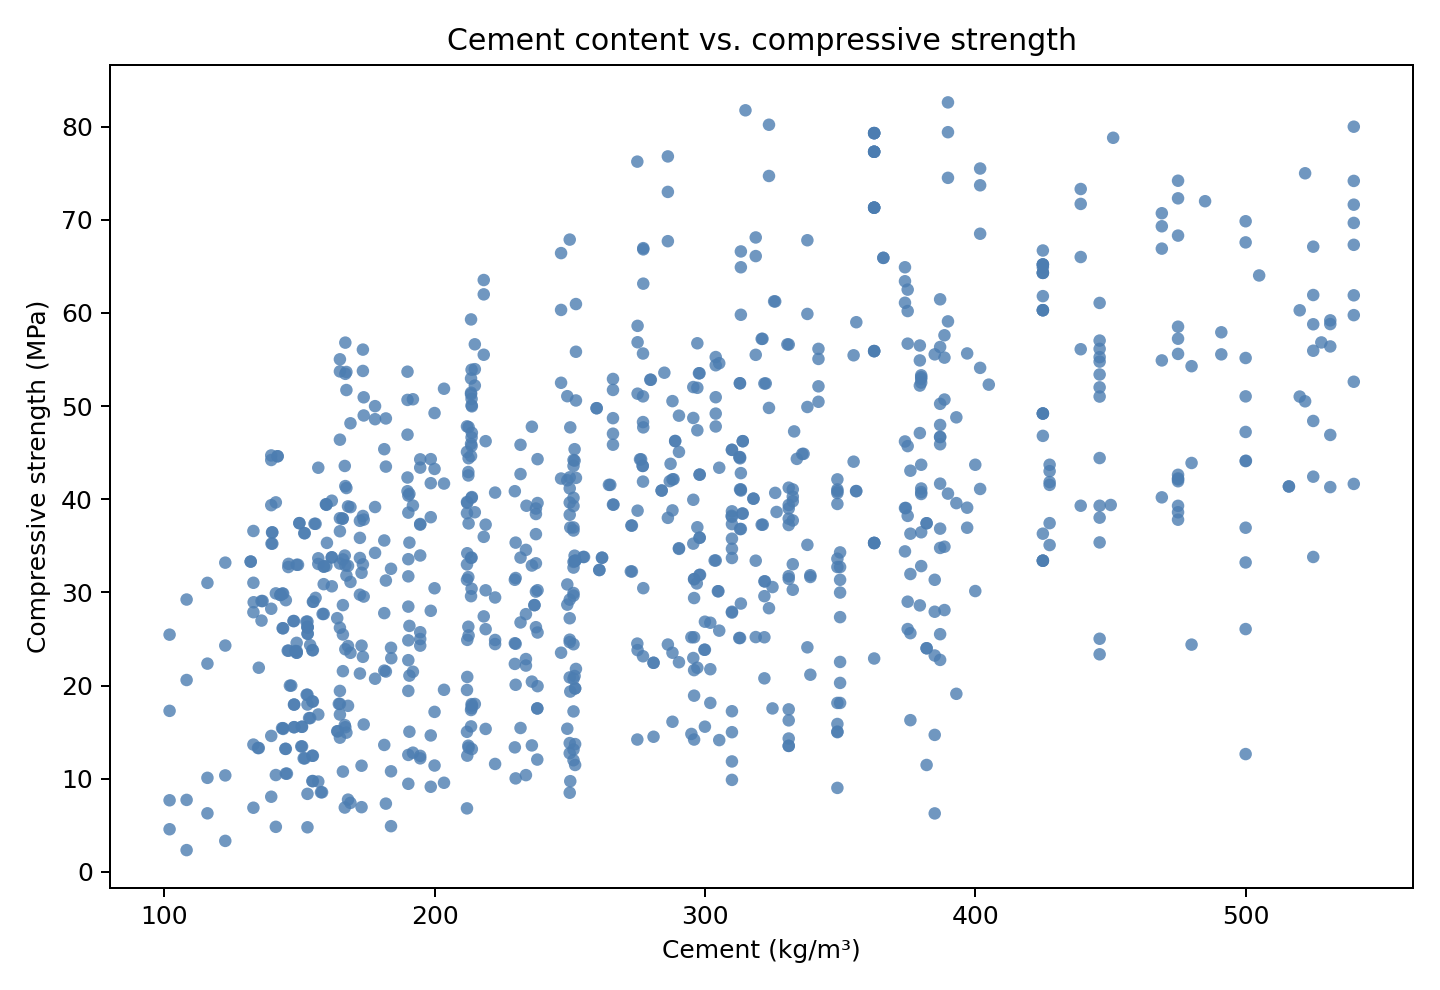
\includegraphics[width=0.75\textwidth]{assets/cement_strength.png}
    \caption{Cement content and measured compressive strength of the concrete samples.}
    \label{fig:cement-strength}
\end{figure}

Additionally, we looked at the relationship between curing age and concrete strength in Figure~\ref{fig:age-strength}, but it didn’t seem like there was much of a correlation.

\begin{figure}[H]
    \centering
    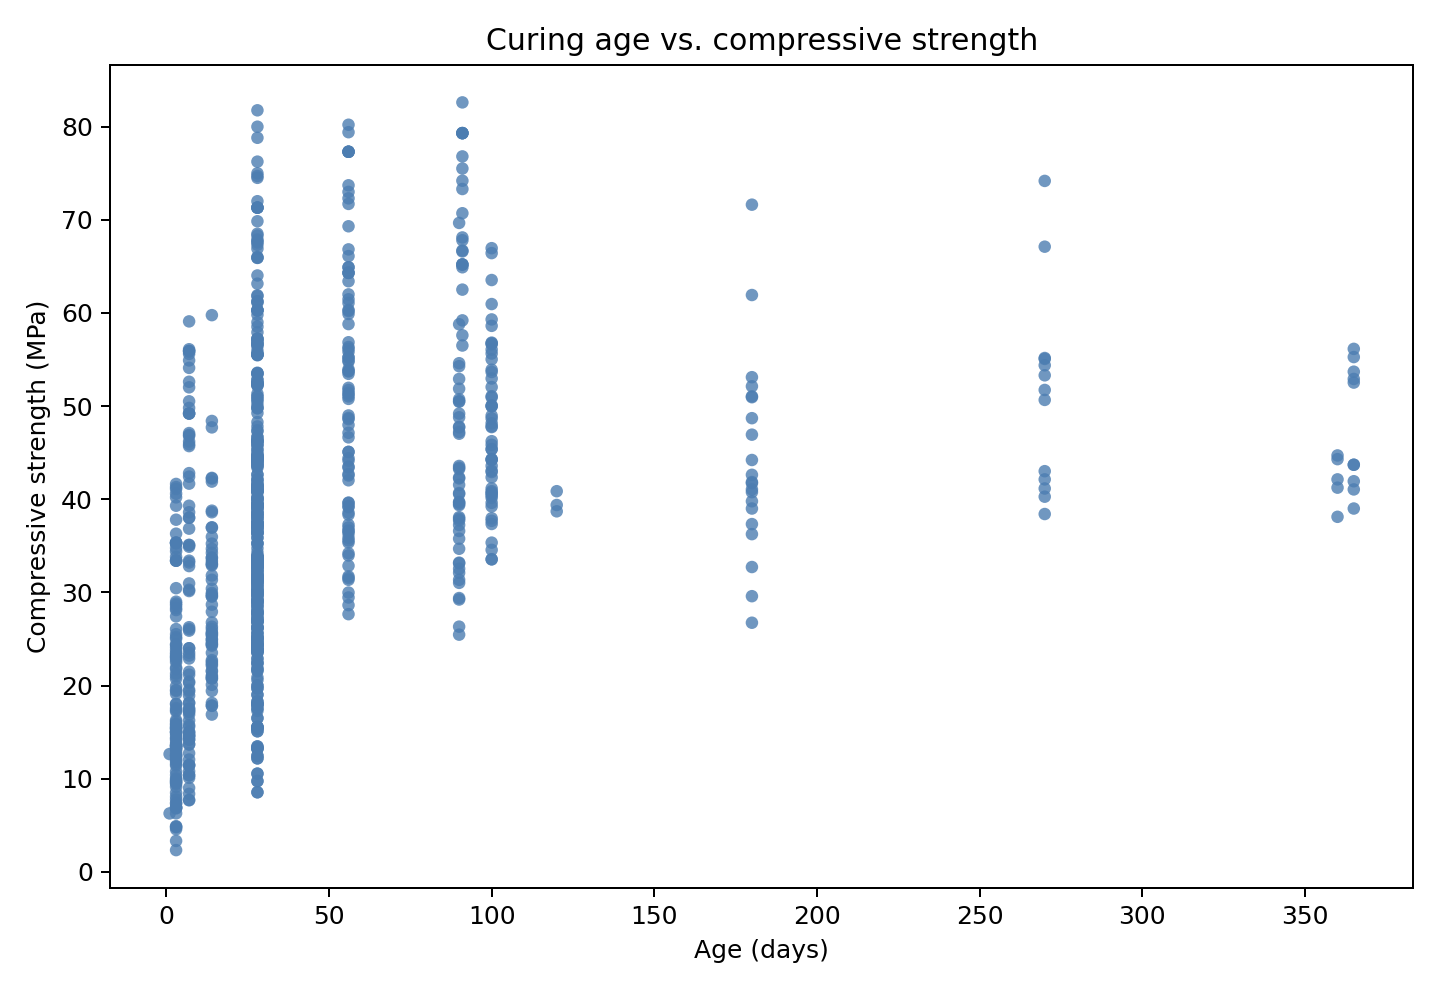
\includegraphics[width=0.75\textwidth]{assets/age_strength.png}
    \caption{Measured compressive strength of concrete samples at different curing ages.}
    \label{fig:age-strength}
\end{figure}

It is clear that there can be drastic variation in strength among concrete mixes of the same cement content or age, showing that one must consider many features holistically in order to more accurately gauge strength.

\newpage

\section{Model Reliability \& Analytical Findings}

The final model explained around 80\% of the variation in strength among training samples, and around 75\% of the variation among testing samples. Since it performed similarly across the two groups, we can conclude it learned relationships that remained useful for samples it hadn’t seen during development. However, since the model can’t explain all of the variation in strength, we suggest supplementing its predictions with physical testing.

The final model log-transforms the inputs, which significantly improved performance compared to the original model. We also tried standardizing the inputs, but it did not lead to any change compared to the original. Table~\ref{tab:model-performance} compares the training and testing performance of all three models.

\begin{table}[H]
    \centering
    \caption{Linear regression performance with original, standardized, and log-transformed inputs, using 900 training observations and 130 testing observations. Higher $R^2$ and lower testing mean squared error (MSE) indicate better performance.}
    \label{tab:model-performance}
    \begin{tabular}{lrrr}
        \toprule
        \textbf{Model} & \textbf{Training $R^2$} & \textbf{Testing $R^2$} & \textbf{Testing MSE (MPa\textsuperscript{2})} \\
        \midrule
        Original inputs & 0.624 & 0.351 & 141.26 \\
        Standardized inputs & 0.624 & 0.351 & 141.26 \\
        Log-transformed inputs & 0.799 & 0.750 & 54.52 \\
        \bottomrule
    \end{tabular}
\end{table}

The original model provides straightforward relationships between ingredient quantities and predicted strength. For example (holding other predictors constant), an additional 10 kg/m\textsuperscript{3} of cement was associated with around 1.33 MPa higher strength. The log scaled model has more complex relationships, but in this case, that allowed it to have more accurate predictions in general.

For practical use, the final model is a useful datapoint for comparing concrete formulations. Its testing root mean squared error is around 7.4 MPa, so individual predictions can still vary from the measured strength. Before using predictions to guide operational changes, the organization should do physical trials and compare the results.

\newpage

\section{Strategic Recommendations \& Implementation Plan}

One recommendation would be that since the p-values of the Cement and Age features are extremely low across all the different models we tested and their coefficients in the untransformed model are positive, that adding a higher proportion of cement as well as simply waiting longer for the concrete to set is an effective method to increase concrete strength. Another recommendation would be to test mixtures with a higher proportion of blast furnace slag, since its coefficient is positive and its p-value is also consistently low across all models. If slag is cheaper than cement, partial cement replacement could reduce costs, provided strength tests confirm that the mix still meets the required strength. Finally, we tested a variety of water/cement ratios across randomly sampled values of the other features, and found their predicted strength according to our best model. This illustrates that generally, our model predicts that 28-day strength increases with decreased water/cement ratio, so an actionable suggestion would be to decrease the amount of water proportional to cement as long as the mixture still holds and while minimizing costs, in order to maximize the strength of the concrete in the long run.

\begin{figure}[H]
    \centering
    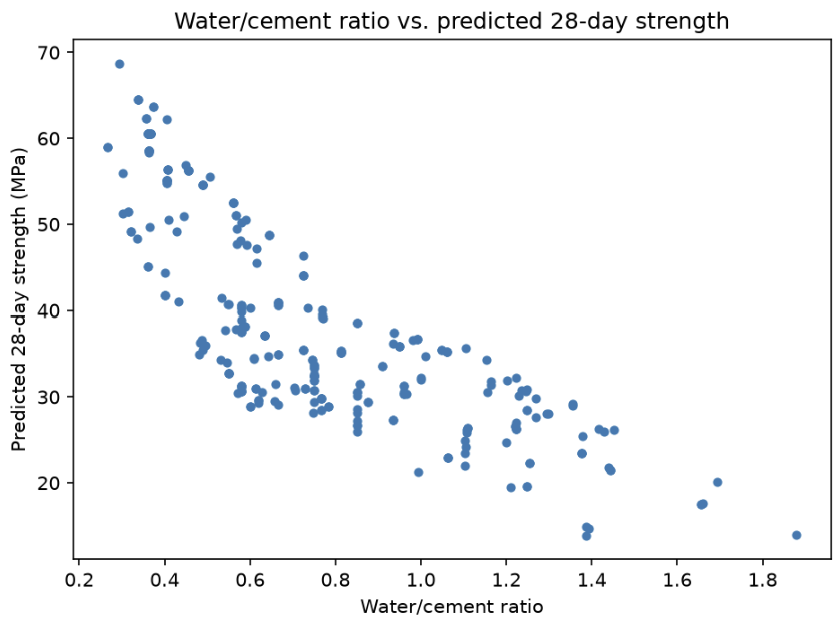
\includegraphics[width=0.75\textwidth]{assets/water_cement_28_day.png}
    \caption{Predicted strength at 28 days for different water/cement ratios, using the log-transformed model.}
    \label{fig:water-cement-strength}
\end{figure}

Figure~\ref{fig:water-cement-strength} shows the predicted 28-day strengths across the sampled water/cement ratios, supporting the recommendation to evaluate mixtures with lower ratios through physical testing.

We acknowledge that there are many potential limitations of our current model. One is the possibility that certain relevant environmental factors are not accounted for, such as temperature or humidity, which could affect concrete strength and cause extra variance that is not able to be accounted for in the training data. A more risk-averse model could be made if more potentially relevant features were tested and evaluated to see if they improve model performance (decided first by consulting with an expert engineer). Our testing of models could also incorporate cross-validation, to ensure that we aren’t overfitting by optimizing for the one specific set of testing data that we initially chose. Also, a linear regression model may not be able to account for all the patterns in the data. This can be mitigated in future model improvements by incorporating nonlinear features, for example a water/cement ratio, or by using nonlinear models such as random forests or polynomial regression.

Finally, one way to ensure our model stays relevant and accurate over long periods of time is implementing a continuous monitoring framework. The first step would be that whenever a construction team affiliated with the project creates a new concrete mix, they should set aside a small portion of that mix for testing. The set-aside mix can then be used to form multiple concrete samples, which can be tested for strength on different days to get multiple training examples with varying ages from just one new mix. The results (the proportion of materials used as well as the age of the concrete mix) can then be logged using a customized data entry system or into a spreadsheet. This can then be hooked up to a database, and on the backend, we can evaluate the current model’s performance on the new entries as well as use the new entries to retrain/refine the existing model to hopefully better fit future concrete mixes. We can do this by training newer models on only a center number of the most recent samples, so that the model is able to adapt to changing conventions in material composition and other changes that might make a model only trained on historical concrete data obsolete.

\end{document}

